%%%%%%%%%%%%%%%%%%%%%%%%%%%%%%%%%%%%%%%%%%

\chapter{Testing of components on the West beamline}\label{chap:fall2021}

%%%%%%%%%%%%%%%%%%%%%%%%%%%%%%%%%%%%%%%%%%

\begin{figure}
\centering
%subfigure width gets "multiplied" by includegraphics width
\begin{subfigure}{.5\textwidth} 
  \centering
  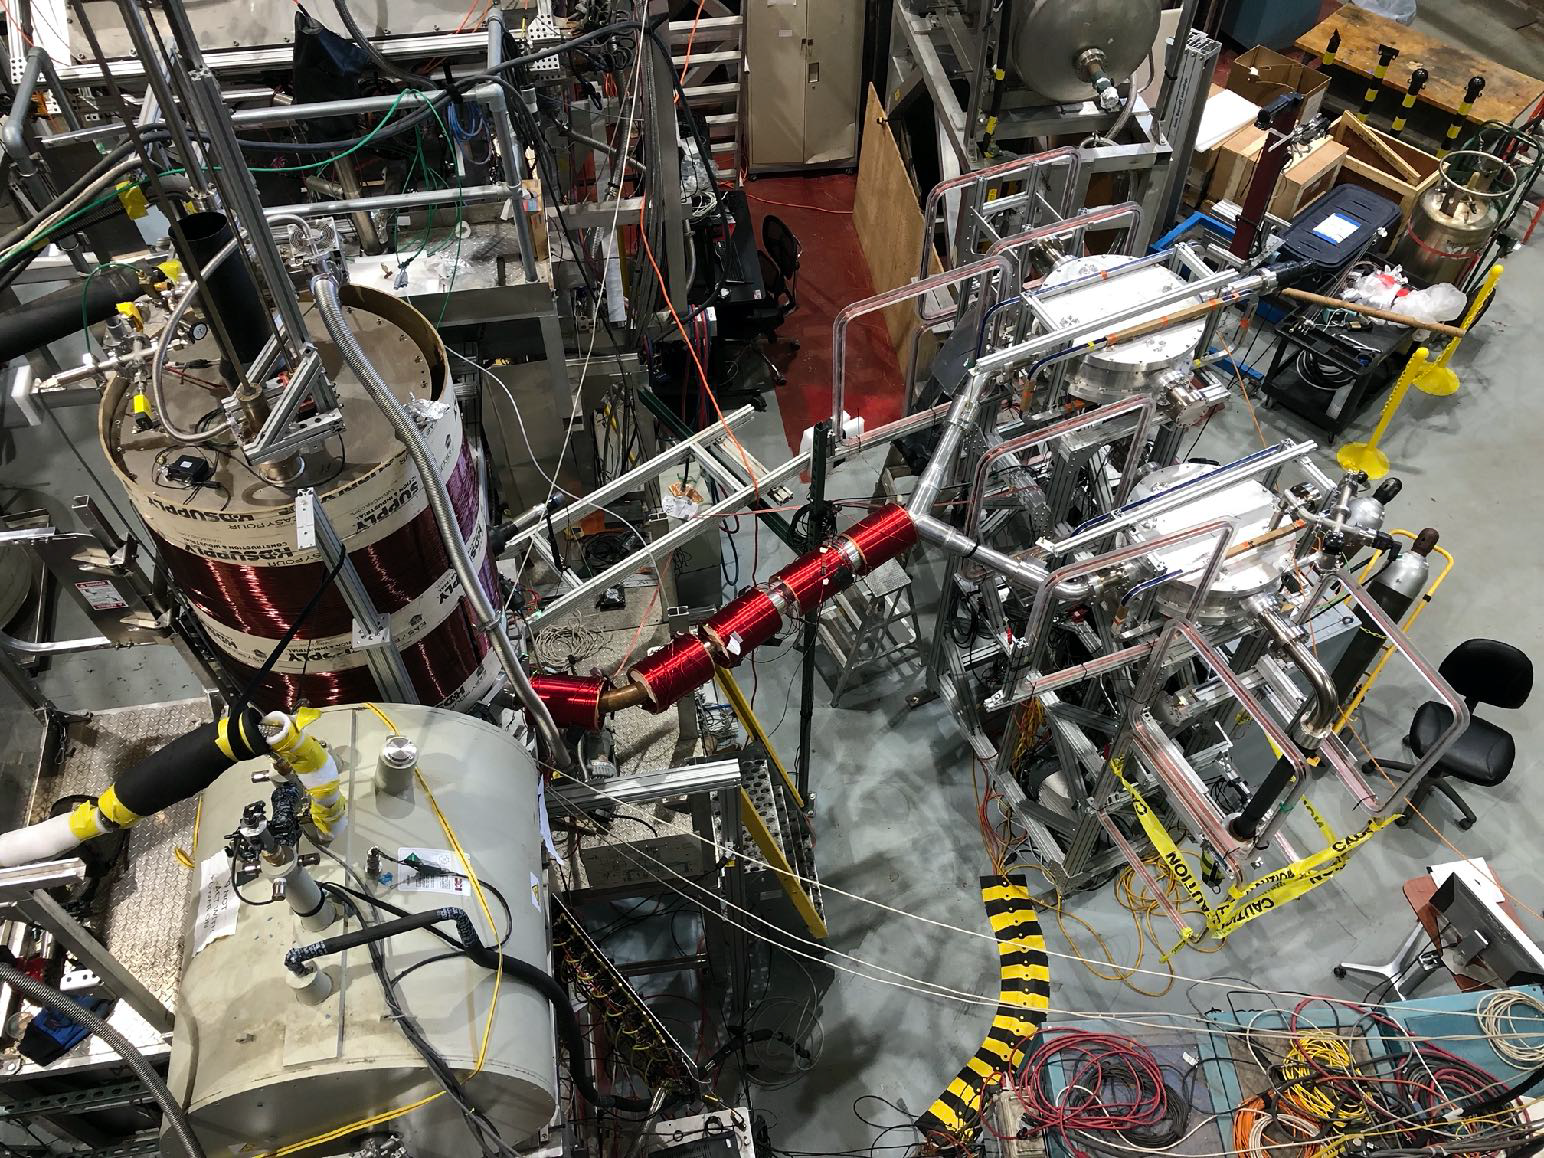
\includegraphics[width=\textwidth]{figures/west_beamline_switcher_tests.png}
  \caption{}\label{subfig:west_beamline_switchers}
\end{subfigure}%DO NOT REMOVE THIS '%'
\begin{subfigure}{.5\textwidth}
  \centering
  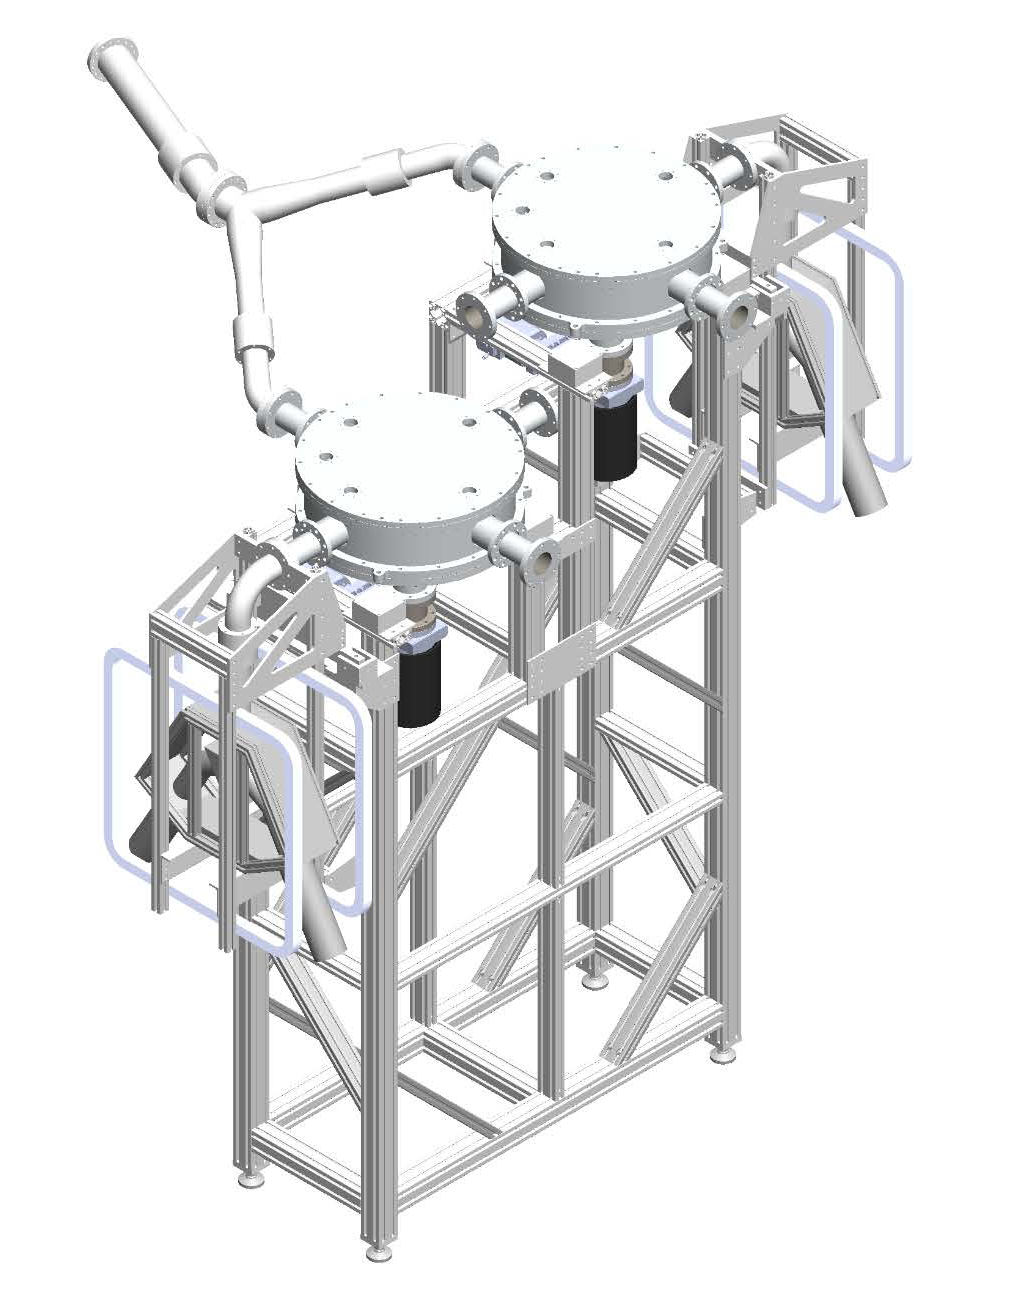
\includegraphics[height=3in]{figures/switcher_mockup.png}
  \caption{}\label{subfig:switcher_mockup}
\end{subfigure}
\caption
{Caption}
\label{fig:west_beamline_switchers}
\end{figure}

% Both PMTs beam height on switcher 1 (higher switcher)
% ======================================================
% SINGLE CHANNEL DET FOIL OUT
% detector rate: 1443.88
% wgv rate: 632.46
% normalized to wgv 650 [Hz]: 1483.9230939506056

% BEAM HEIGHT DET: WEST TEST PORT
% detector rate: 1435.18
% wgv rate: 641.26
% normalized to wgv 650 [Hz]: 1454.7406668122135

% BEAM HEIGHT DET: STRAIGHT THROUGH
% detector rate: 1498.215
% wgv rate: 635.39
% normalized to wgv 650 [Hz]: 1532.6645839563103

% Beam height PMTs on both switchers
% ======================================================
% SINGLE CHANNEL DET FOIL OUT
% detector rate: 1465.2666666666667
% wgv rate: 656.6
% normalized to wgv 650 [Hz]: 1450.5381256980404

% BEAM HEIGHT DET: SWITCHER 2 (LOWER)
% detector rate: 2244.225
% wgv rate: 650.0416666666666
% normalized to wgv 650 [Hz]: 2244.0811486443176

% BEAM HEIGHT DET: SWITCHER 1 (HIGHER)
% detector rate: 1512.1142857142856
% wgv rate: 649.5142857142857
% normalized to wgv 650 [Hz]: 1513.2450622443143

% Switcher 2 transmission difference: 1.5425987599300384